% ML4H 2026 submission — Proceedings track.
% Compile with the official ML4H 2026 template (jmlr.cls + ml4h macros) from Overleaf:
%   https://www.overleaf.com/latex/templates/machine-learning-for-health-ml4h-2026-template
% Drop this file in as main.tex. See README.md for the two-line change that switches
% this to the 4-page Findings track.
\documentclass[pmlr,twocolumn,10pt]{jmlr}

\mlhtrack{proceedings}

\newif\iffinal
\finalfalse   % \finaltrue for camera-ready (de-anonymises authors)

\usepackage{booktabs}
\usepackage{multirow}
\usepackage{graphicx}

\title[Guardrails Do Not Generalise]{Guardrails Do Not Generalise: Five Measured Safety
and Evaluation Failures in a Clinical ECG Explanation System}

\iffinal
  \author{\Name{Author Name} \Email{author@institution.edu}\\
  \addr Institution}
\else
  \author{Anonymous Author(s)}
\fi

\begin{document}

\maketitle

\begin{abstract}
Clinical machine-learning systems are usually reported as models, but they are deployed as
pipelines, and their safety properties live in the pipeline rather than in the model. We
build a 12-lead ECG interpretation system on PTB-XL whose generated explanations are
constrained by a mechanical consistency gate: the report may assert only findings the
detector surfaced. We then extend the system five times --- with retrieval, human feedback,
synthetic augmentation, Spanish output, and a rare-class evaluation --- and measure what
happens to the guarantee each time. In every case a property that held before the extension
silently failed afterwards, and in no case was the failure visible in the system's own
outputs. Retrieval-augmented generation \emph{doubled} the hallucination rate
($0.060 \rightarrow 0.120$) in a task where the model is forbidden to add findings.
Threshold updates from reviewer feedback moved in one direction only (9 up, 0 down) and
cost $2.1\%$ macro-F1; allowing reviewers to report missed findings did not fix it
(10 up, 0 down), while sampling below the decision threshold did ($+10.3\%$). Adding
Spanish reduced fabricated-finding detection from $100\%$ to $0\%$, because the gate matched
English strings. On the 17 rarest labels, the bootstrap confidence interval customarily
reported is $4.0\times$ \emph{narrower} than the analytic one, concealing that those labels
have a median of two positive test cases. Synthetic augmentation degraded every arm below
baseline, from a generator that passed every standard sample-quality check while producing
QRS complexes twice their true width. We argue that clinical ML needs guardrail
\emph{regression testing} --- each of these failures is trivially detectable by a test that
nobody writes.
\end{abstract}

\begin{keywords}
electrocardiography, clinical decision support, hallucination, evaluation methodology,
negative results, retrieval-augmented generation, health equity
\end{keywords}

\section*{Data and Code Availability}
This work uses PTB-XL \citep{wagner2020ptbxl}, a public, de-identified 12-lead ECG dataset
of 21{,}799 records from 18{,}869 patients, distributed under CC BY 4.0 via PhysioNet. No
private or institutional data was used. All code, configurations, and the artefacts behind
every number reported here are released under an open licence; the repository is withheld
during review for anonymity and an anonymised copy is available to reviewers on request.

\section*{Institutional Review Board (IRB)}
This study used only a public, fully de-identified dataset and involved no human subjects,
no prospective data collection, and no clinical deployment. IRB approval was therefore not
required.

\section{Introduction}

A clinical ML paper typically reports a model: an architecture, a training procedure, and a
table of discrimination metrics. What a hospital deploys is a pipeline --- a detector, a
report generator, a review interface, an integration layer --- and the properties clinicians
rely on are properties of that pipeline. ``The system never asserts a finding it did not
detect'' is not a fact about a neural network. It is a fact about a parser, a vocabulary,
and a comparison, and it holds only as long as those keep matching the thing they were
written against.

This paper is about what happens when they stop. We built an ECG interpretation system whose
central safety property is a \emph{consistency gate}: generated explanations are parsed back
into the set of conditions they assert, and any report asserting a finding the detector did
not surface is flagged before a clinician sees it. The gate is mechanical, cheap, and it
works. We then extended the system in five ordinary directions --- adding retrieval, a
human-feedback loop, synthetic training data, a second language, and a rare-class evaluation
--- and instrumented what the extension did to the guarantee.

Every extension broke something, and none of the breakages were visible in the output. A
Spanish report that invents a diagnosis is fluent, well-formed, carries the disclaimer, and
passes the gate. A feedback loop that is quietly destroying recall shows rising precision on
every dashboard. A rare-class result with a tight-looking confidence interval is resting on
two patients.

\paragraph{Contributions.}
\begin{enumerate}
\item \textbf{Retrieval increases hallucination when assertions are constrained}
(\S\ref{sec:rag}). Over 150 paired records, adding retrieved reference text doubled the
hallucination rate, $0.060 \rightarrow 0.120$. The mechanism is instrumented, not inferred.
\item \textbf{Feedback loops ratchet} (\S\ref{sec:feedback}). Feedback on surfaced findings
contains false positives and no false negatives, so thresholds can only rise. Reviewer-reported
misses --- the intuitive fix --- do not help; sub-threshold sampling does.
\item \textbf{Safety gates are language-bound} (\S\ref{sec:i18n}). Adding Spanish took
fabricated-finding detection from $100\%$ to $0\%$ for Spanish-speaking patients only.
\item \textbf{Rare-class evaluation is underpowered, and the standard interval hides it}
(\S\ref{sec:power}). On PTB-XL's 17 rarest labels the record bootstrap reports intervals
$4.0\times$ narrower than Hanley--McNeil.
\item \textbf{A generator can pass every sample-quality check and still be unusable}
(\S\ref{sec:synth}). Ours showed no memorisation and no mode collapse while emitting QRS
complexes of 227\,ms against a true 112\,ms.
\item \textbf{Differencing halves performance} (\S\ref{sec:longitudinal}), and the cohort
that looks like a natural control for it is the sickest cohort in the dataset.
\end{enumerate}

We do not claim state-of-the-art detection: our detector reaches 0.9199 macro-AUROC against
0.925 for the best published PTB-XL baseline \citep{strodthoff2021deep}. The contribution is
the failure analysis, and it is only possible \emph{because} the system is otherwise ordinary.

\section{System}
\label{sec:system}

\begin{table}[t]
\centering
\caption{System components. Every figure is on PTB-XL's official test fold (fold 10,
$n=2{,}198$) except the subgroup rows, which are bootstrap estimates over 200 replicates.}
\label{tab:system}
\small
\begin{tabular}{lc}
\toprule
\textbf{Detection} (71 labels) & macro-AUROC \\
\midrule
This work (1D ResNet, 8.78M) & 0.9199 \\
Best published \citep{strodthoff2021deep} & \textbf{0.9250} \\
\midrule
\textbf{Calibration} & ECE \\
\midrule
Uncalibrated & 0.0793 \\
Temperature scaling & 0.0875 \\
Per-label temperature & 0.0890 \\
Per-label vector scaling & \textbf{0.0020} \\
\midrule
\textbf{Distillation} & AUROC (size) \\
\midrule
Teacher & 0.9199 (35.2\,MB) \\
Student, distilled & 0.9174 (1.05\,MB) \\
Student, from scratch & 0.9029 (1.05\,MB) \\
Larger student, distilled & \textbf{0.9219} (3.99\,MB) \\
\midrule
\textbf{Subgroup} & macro-AUROC \\
\midrule
Male ($n=1{,}132$)   & 0.925 [0.914, 0.934] \\
Female ($n=1{,}066$) & 0.906 [0.896, 0.919] \\
Gap & \textbf{0.0188 [0.0044, 0.0325]} \\
\bottomrule
\end{tabular}
\end{table}

\paragraph{Detection.} A 1D residual CNN (8.78M parameters) over the 12-lead, 10\,s, 100\,Hz
signal, trained multi-label over PTB-XL's 71 SCP-ECG statements with the official
patient-level folds (train 1--8, validation 9, test 10). Test macro-AUROC is 0.9199 over 71
labels and 0.8929 over the five diagnostic superclasses, against 0.925 for the strongest
published architecture on the same split \citep{strodthoff2021deep}. This is a competent but
not novel detector, which is the point: the failures below are not artefacts of a weak model.

\paragraph{Calibration.} Raw sigmoid outputs are badly calibrated (ECE 0.0793). Temperature
scaling \citep{guo2017calibration} does not fix it and in fact makes it slightly
\emph{worse} (0.0875), as does a per-label temperature (0.0890): temperature can only
sharpen or soften a distribution, and the dominant error here is a \emph{bias} introduced by
class-weighted training. Per-label \emph{vector} scaling --- an affine transform of each
logit, which can shift as well as scale --- reduces ECE to 0.0020 and cuts spuriously
surfaced labels from 7.4 to 1.9 per record. Every transform is monotone per label, so AUROC
is unchanged at 0.9199 throughout.

\paragraph{Explanation and the consistency gate.} A deterministic templater renders the
detected findings into a two-section clinical report. The gate parses generated text back
into the set of SCP conditions it asserts and compares that set against what the detector
surfaced; anything asserted but not surfaced is an unsupported claim. Because the templater
renders only from the detections, it is consistency-clean by construction --- which is what
makes it a useful control for measuring what an LLM backend does to the property.

\paragraph{Distillation.} Knowledge distillation \citep{hinton2015distilling} to a
253{,}895-parameter student (1.05\,MB, $34\times$ fewer parameters) retains 0.9174 AUROC, against
0.9029 for the same architecture trained from scratch --- a 1.4-point gain attributable to
distillation rather than architecture, since every student was trained both ways. A
988{,}487-parameter student reaches 0.9219, \emph{exceeding} its teacher, indicating the
deployed model is over-parameterised for this task.

\paragraph{Subgroup performance.} Macro-AUROC is 0.925 [0.914, 0.934] for male and
0.906 [0.896, 0.919] for female patients; the gap of 0.0188 [0.0044, 0.0325] excludes zero
over 200 bootstrap replicates. We report this as an unresolved defect rather than a solved
problem \citep{obermeyer2019dissecting}.

\section{Finding 1: Retrieval doubles hallucination}
\label{sec:rag}

We added retrieval-augmented generation \citep{lewis2020retrieval} over a 927-passage corpus
of openly-licensed cardiology reference text, retrieving per detected finding and injecting
the passages into the generator's prompt. The generator's contract forbids asserting any
condition not in the structured input.

Over 150 test records generated twice under greedy decoding --- identical input, identical
prompt except the retrieved block --- retrieval made every faithfulness metric worse
(Table~\ref{tab:rag}).

\begin{table}[t]
\centering
\caption{Retrieval on a constrained-assertion task, 150 paired records, greedy decoding.}
\label{tab:rag}
\begin{tabular}{lcc}
\toprule
 & no RAG & RAG \\
\midrule
Hallucination rate     & \textbf{0.060} & 0.120 \\
Consistency rate       & \textbf{0.940} & 0.880 \\
Well-formed rate       & \textbf{0.700} & 0.540 \\
Banned treatment recs. & \textbf{0.180} & 0.447 \\
Finding coverage       & 0.342 & \textbf{0.414} \\
\bottomrule
\end{tabular}
\end{table}

McNemar's exact test over discordant pairs (5 hallucinating only without RAG, 14 only with)
gives $p = 0.064$: directionally clear, short of significance, and reported as such.

The mechanism is specific and was instrumented rather than assumed. For every fabricated
finding we checked whether that condition was named in \emph{that record's} retrieved
passages. Left ventricular hypertrophy was fabricated 8 times under RAG and all 8 had LVH
named in the retrieved context, against 3 times without. ST elevation, by contrast, was
fabricated in both arms and never appeared in the context --- that one is the model's prior,
and an aggregate hallucination count would have silently credited retrieval with the
difference.

The lesson is not that retrieval is harmful. It is that retrieval supplies \emph{plausible
condition names}, and in a task whose safety property is ``assert only what was detected'',
condition names are exactly the contaminant. Retrieval belongs on the wording, not on the
assertions.

\section{Finding 2: Feedback loops ratchet}
\label{sec:feedback}

We built a reviewer interface (rate each finding correct/incorrect/uncertain, report what was
missed), a local store, and a policy that turns ratings into per-label decision thresholds
using a Beta posterior anchored on the model's own calibrated confidence.

A reviewer can only rate findings the system \emph{showed} them. Every rating is therefore
drawn from above the current threshold, where the only visible error is a false positive.
Raising a threshold is always supported by such data; lowering one never is.

We measured this with a reviewer simulated from PTB-XL labels, streaming feedback from the
validation fold and scoring on test (Table~\ref{tab:feedback}).

\begin{table}[t]
\centering
\caption{Online threshold updates. Direction of movement is the diagnostic; F1 is macro over
71 labels on the held-out test fold.}
\label{tab:feedback}
\begin{tabular}{lccc}
\toprule
Arm & up & down & $\Delta$F1 \\
\midrule
A: no feedback              & --- & --- & --- \\
B: ratings only             & 9  & \textbf{0}  & $-0.0045$ \\
C: + reported misses        & 10 & \textbf{0}  & $-0.0045$ \\
D: + sub-threshold sampling & 1  & \textbf{18} & $\mathbf{+0.0221}$ \\
E: D, 10\% reviewer error   & 1  & 19 & $+0.0199$ \\
\bottomrule
\end{tabular}
\end{table}

Arms B and C moved 19 thresholds between them and not one downward. The result worth
pausing on is C: letting clinicians report missed findings is the intuitive remedy, it
collected 1{,}647 reported misses, and it changed nothing --- performance matched B to four
decimal places. Knowing a true positive lies below the threshold says nothing about how many
false positives lie beside it, so it still cannot justify lowering anything. Recall evidence
and precision evidence are different quantities and only one had been collected.

\begin{figure}[t]
\centering
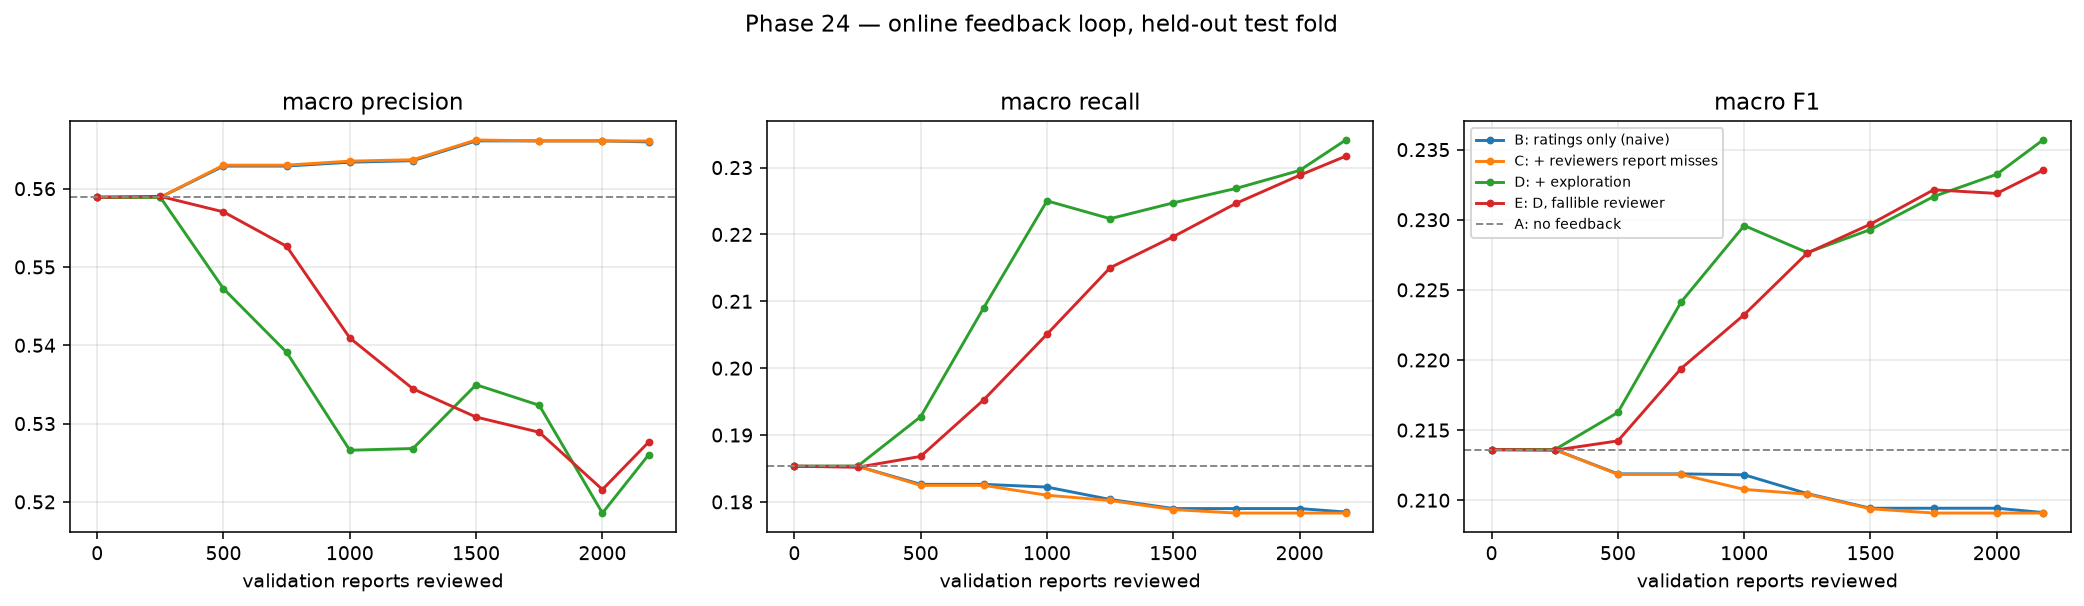
\includegraphics[width=\linewidth]{loop.png}
\caption{Held-out macro precision, recall and F1 as reviewer feedback accumulates. Arms B
and C raise precision while recall decays; only the arm that samples below the decision
threshold (D) improves F1. The dashed line is the no-feedback baseline.}
\label{fig:loop}
\end{figure}

Deliberately surfacing $\sim$10\% of sub-threshold findings for review reverses the direction
and yields $+10.3\%$ relative macro-F1, and retains $+9.3\%$ under a reviewer who is wrong
10\% of the time and reports only a third of misses.

\section{Finding 3: Safety gates are language-bound}
\label{sec:i18n}

We added Spanish clinical explanations, motivated by documented language-access disparities
in care. The consistency gate matches English impression phrases. Pointed at a Spanish
report it matches nothing --- so the report parses as asserting \emph{no findings}, which is
a subset of anything, and passes unconditionally.

Over 400 records, a fabricated finding appended to each report was detected in $100\%$ of
English reports and $0\%$ of Spanish ones. A Spanish report inventing \emph{bloqueo completo
de rama izquierda} for a patient whose only detected finding was atrial fibrillation was
reported consistent; the identical English fabrication was caught.

Nothing about the output revealed this. The Spanish text is fluent, correctly sectioned,
carries the disclaimer, and validates against the output schema. Only the guardrail is
absent, and only for those patients. After adding language-aware parsing (accent-folding on
input, longest-match term resolution, and restriction to the impression section) both
languages reach $100\%$ detection and $100\%$ findings round-trip.

We note the generality: any language-bound check --- a keyword filter, a regular-expression
safety rule, a parser --- is a candidate for this failure the moment a second language is
added, and the failure is silent by construction.

\section{Finding 4: Rare-class intervals conceal their own weakness}
\label{sec:power}

Rare-class performance is a standard claim in clinical ML. On PTB-XL it is largely
unmeasurable, and the interval usually reported does not say so.

The 17 labels with fewer than 50 training examples have a \emph{median of two positive cases}
in the official test fold. A percentile bootstrap over test records reports these labels as
measured \emph{more tightly} (median 95\% CI width 0.035) than well-supported labels (0.041)
--- because with two positives every resample reuses the same two patients and merely
reshuffles 2{,}196 negatives. It cannot resample the quantity that is scarce. The analytic
Hanley--McNeil standard error \citep{hanley1982meaning}, which depends explicitly on the
positive count, puts the same labels at a median CI width of \textbf{0.373}, $4.0\times$
wider.

We flag this because the failure is self-concealing: the narrower interval is the one
produced by the more modern-sounding method, and a rare-class improvement reported with it
will look better supported than one reported honestly.

\section{Finding 5: Sample-quality checks miss what matters}
\label{sec:synth}

We trained a conditional 1D diffusion model \citep{ho2020denoising} to generate ECGs for
rare classes, and compared five augmentation strategies under induced rarity (50 real
examples retained per target label; every arm adding an identical 350 rows per label).

Every arm scored below the un-augmented baseline (macro-AUROC over 8 targets: baseline
0.8960; oversampling 0.8733; classical augmentation 0.8810; synthetic 0.8776;
synthetic+classical 0.8829), and all arms also degraded the other 63 labels.

The generator passes the checks such work usually reports: nearest-neighbour distance ratio
1.08 against held-out real data (no memorisation), diversity ratio 1.11 (no mode collapse),
and $100\%$ of samples yielding a delineable QRS complex. Measured against the same
delineator the system uses clinically, it fails the check that matters:

\begin{center}
\begin{tabular}{lcc}
\toprule
 & synthetic & real \\
\midrule
QRS duration    & 227\,ms & 112\,ms \\
PR interval     & 222\,ms & 183\,ms \\
P wave detected & 31\% & 85\% \\
\bottomrule
\end{tabular}
\end{center}

The model learned the low-frequency envelope of an ECG and not the sharp deflections that
carry the diagnosis. That explains the direction of the result rather than merely
accompanying it: the target classes are \emph{defined} by the morphology the generator gets
wrong --- bundle branch block is a wide QRS, and a premature atrial contraction is a
premature P wave in a generator that produces a detectable P only 31\% of the time. These
samples do not add weak examples of the class; they add examples that contradict its
definition.

\section{Finding 6: Differencing halves performance}
\label{sec:longitudinal}

Serial comparison --- what changed since the prior ECG --- drives more clinical decisions
than the absolute reading does. We built it on the 2{,}930 prior/current record pairs PTB-XL
contains, and measured what differencing costs.

On 294 held-out pairs, the \emph{same} detector scores macro-F1 0.640 on ``what is present''
and 0.322 on ``what is new'' (precision 0.478, recall 0.242). Differencing two independent
threshold crossings roughly doubles the error rate; the difficulty is not that change is
subtler, but that a difference of two noisy decisions is noisier than either.

Establishing a noise floor for that comparison exposed a second trap. The obvious null
cohort --- 327 pairs recorded under 24 hours apart, too soon for real remodelling --- is not
one. Its measured spread is \emph{larger} than that of pairs a year apart (QRS SD 40.8\,ms
vs 27.1\,ms), which noise cannot do. Same-day repeat ECGs select for acutely unwell patients:
63\% carry an acute or arrhythmic code against 34\% of year-apart pairs. The cohort that
looks like a null is the sickest cohort in the dataset.

We also note that 73\% of same-patient pairs differ in their annotated label set, and this
holds at \emph{zero} elapsed time (72\% for pairs under 24 hours apart). Any evaluation
treating an annotation difference as ground truth for clinical change inherits that noise.

\section{Specialist versus generalist}
\label{sec:benchmark}

For context we benchmarked against a general-purpose LLM given the \emph{same} intervals our
own delineator extracts --- a deliberately generous protocol, since the model never has to
find a QRS complex. On the five superclasses the specialist reaches 0.8929 macro-AUROC at
5\,ms per record; the generalist reaches 0.4681, with every per-class confidence interval
containing 0.5 (no measurable discrimination), at 4{,}387\,ms. Projected from measured token
counts at list prices, a hosted frontier model would cost $\sim$\$2.07 per 1{,}000
inferences against \$0.0001 locally, before the column that decides clinical deployments:
whether patient data leaves the host.

We did not run a frontier multimodal model --- no API credentials were available --- and
record that rather than substituting a proxy. Published image-based GPT-4o ECG accuracy
($\sim$41\% multiclass, \citealp{zaboli2025gpt4o}) is cited, not measured here.

\section{Related work}

PTB-XL \citep{wagner2020ptbxl} and its benchmark suite \citep{strodthoff2021deep} are the
standard setting for ECG classification; large-scale supervised ECG models
\citep{ribeiro2020automatic} established the task's feasibility. Our detector is deliberately
conventional. Calibration \citep{guo2017calibration} and distillation
\citep{hinton2015distilling} are applied as published. The contribution here is orthogonal to
model quality: it concerns whether pipeline-level guarantees survive pipeline-level change,
which to our knowledge is not systematically measured in clinical ML.

\section{Limitations}

Findings 2 and 5 use simulated rather than human reviewers and clinician review
respectively, and Finding 2's ``ground truth'' is PTB-XL's own annotation, which we
separately measured as unstable (72\% of same-patient record pairs differ in their annotated
label set at zero elapsed time). Finding 1 is one generator, one corpus, and one prompt at
$p=0.064$. Finding 5 is one generator family at one training budget and one rarity level.
Finding 3's Spanish vocabulary is validated mechanically against Spanish cardiology prose
(34 of 67 terms confirmed) but has not been reviewed by a Spanish-speaking cardiologist. The
generalist comparison uses a small local model, not a frontier one. All results are on a
single public dataset from a single European cohort, and none of this system has been
deployed or evaluated prospectively.

\section{Conclusion}

Each failure reported here is trivially detectable --- by a test asserting that the gate
catches a fabricated finding in every supported language; by a check on the direction of
threshold movement; by an interval whose width depends on the number of positive cases; by
measuring whether synthetic ECGs have physiologic intervals. None of these tests is
difficult. What they have in common is that the property they protect was established once,
early, in a narrower system, and nothing re-checked it when the system grew.

We suggest that clinical ML pipelines need \emph{guardrail regression tests} in the same
sense software has regression tests: an executable assertion, run on every change, that the
safety property still holds --- including for the inputs, languages, and populations added
since it was written. Reporting a safety mechanism once, in the paper that introduces it, is
not evidence that it still functions in the system that ships.

\bibliography{references}

\end{document}
